% ----------------------------------------------------------
\chapter{Modelo mecânico}
% ----------------------------------------------------------

Esse capítulo traz uma descrição geral do modelo mecânico que será utilizado neste trabalho. Portanto, são apresentadas as equações de equilíbrio e constitutivas que foram utilizadas, sem aprofundar, no entanto, nas particularidades que compreendem o domínio de um túnel profundo. Essas serão vistas no final do Capitulo 6, após a descrição da solução desse modelo mecânico. 

\section{Equações de Equilíbrio local e a hipótese da evolução quase estática}

A segunda lei fundamental do equilíbrio dinâmico, ou seja, o princípio da conservação do momento linear, aplicada sobre um subdomínio contínuo $\Omega'$, exige que para $\forall \Omega' \subset \Omega$:

\begin{equation}
	\label{eq:conservacao_momento_linear}
\int_{\Omega'}\rho(\underline\gamma-\underline f)d\Omega' = \int_{\partial\Omega'}\underline T dS
\end{equation}

sendo $\rho$ a densidade do domínio, $\underline\gamma$ o campo de acelerações referente às forças inerciais, $\underline f$ o campo de acelerações referente às forças de corpo (por exemplo, a gravidade) e $\underline T$ o vetor tensão que atua na superfície $dS$ contida na superfície $\partial\Omega'$ de $\Omega'$ (\autoref{subsistema_material}).
%
\begin{figure}[H]
	\begin{center}
		\includegraphics[scale = 1.0]{0501-subsistema no sistema material forças de corpo.pdf}
	\end{center}
	\caption{\label{subsistema_material}Subsistema material $\Omega'$ no interior de um sistema material $\Omega$ submetido a um campo de forças de corpo}
\end{figure}

Considerando a definição $\underline T = \underline{\underline\sigma}\cdot \underline n$ , em que $\underline n$ é o vetor normal à superfície $dS$ e $\underline{\underline\sigma}$ o tensor de tensões, aplicando o teorema da divergência no termo à direita da igualdade (\ref{eq:conservacao_momento_linear}) pode-se escrever que

\begin{equation}
	\label{teorema_divergencia}
	\forall \Omega' \subset \Omega ~~~~ \int_{\Omega'}\left( \underline \nabla \cdot \underline{\underline\sigma}+ \rho(\underline\gamma-\underline f) \right)d\Omega' = \underline 0
\end{equation}

e, portanto,

\begin{equation}
	\label{eq:resultado_teorema_divergencia}
	 \underline \nabla \cdot \underline{\underline\sigma}+ \rho(\underline\gamma-\underline f) = \underline 0
\end{equation}

em que $\nabla \cdot$ é o operador divergente. Aplicando a hipótese de evolução quase estática, ou seja, $\underline\gamma = \underline 0$, tem-se o seguinte sistema de equações de equilíbrio estático local:

\begin{equation}
	\label{eq:equilibrio_estatico_local}
	\underline \nabla \cdot \underline{\underline\sigma}+ \rho \underline f = \underline 0
\end{equation}

Salienta-se também que devido a conservação do momento angular tem-se que o tensor de tensões é simétrico, ou seja, $\underline{\underline\sigma} = \underline{\underline\sigma}^T$ e o sistema (\ref{eq:equilibrio_estatico_local}), em três dimensões, possui 3 equações e 6 incógnitas de tensões.

\section{Admissibilidade estática, natureza Euleriana do Campo de Tensões, Transformação geométrica e medida de deformação}

Para que o sistema material $\Omega$ da \autoref{sistema_material_contorno} esteja em equilíbrio, ou seja, \textbf{estáticamente admissível (E.A)}, o campo de tensões deve satisfazer as equações de campo de equilíbrio local, conjuntamente com as condições de continuidade interna e de contorno (relativo ao princípio da ação-reação) representadas por (\ref{eq:EA}).

\begin{figure}[H]
	\begin{center}
		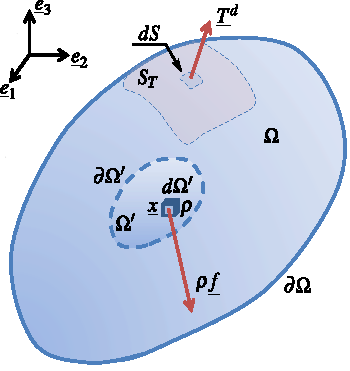
\includegraphics[scale = 1.0]{0502-sistema material com condição de contorno.pdf}
	\end{center}
	\caption{\label{sistema_material_contorno}Sistema material $\Omega'$ com condição de contorno $\underline T^d$ imposta na fronteira $S_T$}
\end{figure}

\begin{equation}
	\label{eq:EA}
	\underline{\underline\sigma}~~ \text{é E.A.} \leftrightarrow \left\{
		\begin{matrix}
			\text{eqs. campo:} \left\{
				\begin{matrix}
					\underline \nabla \cdot \underline{\underline\sigma}+ \rho \underline f = \underline 0 \\ 
					\underline{\underline\sigma} \cdot \underline n ~~ \text{contínuo ao longo de} ~~ \Sigma
		
				\end{matrix}\right. \\ 
			\text{cond. contorno:}~~ \underline{\underline\sigma} \cdot \underline n = \underline T^d ~~ \text{em} ~~ \forall \underline x \in S_T \subset \partial \Omega
		\end{matrix}\right.
\end{equation}

Em que $\Sigma$  representa as superfícies de descontinuidades de $\underline{\underline \sigma}$ no interior do corpo, se houver. A rigor o campo de tensões $\underline{\underline \sigma}$ que satisfaz (\ref{eq:EA}) se refere sempre à configuração atual durante a evolução do sistema, ou seja, possui uma natureza Euleriana (conforme Figura 5.3).

\begin{figure}[H]
	\begin{center}
		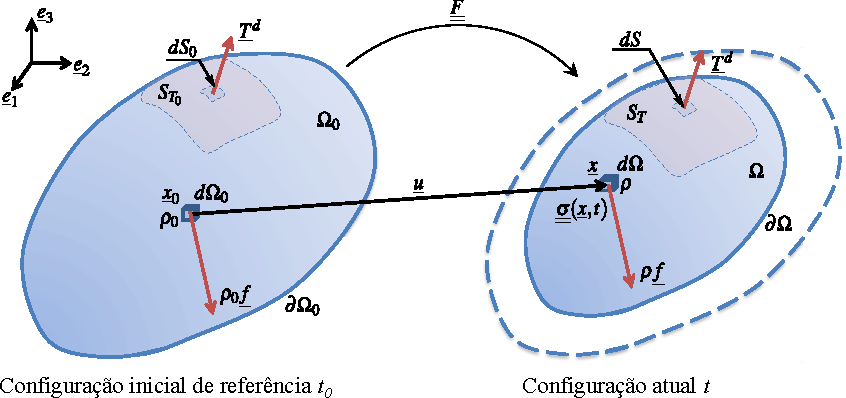
\includegraphics[scale = 1.0]{0503-descricao euleriana do campo de tensoes.pdf}
	\end{center}
	\caption{\label{tensoes_Euleriana}Natureza Euleriana do campo de tensões}
\end{figure}

O vetor $\underline u = \underline x - \underline x_0$ é o deslocamento da partícula durante a evolução do sistema e $\underline{\underline F}$ é o gradiente da transformação geométrica que associa a posição de cada partícula $\underline x_0$ a sua posição $\underline x$ na configuração atual, definido por:

\begin{equation}
	\label{eq:transformacao_geometrica}
 	\underline{\underline F} = \nabla \underline x = \nabla \left( \underline x_0+\underline u \right) = \underline{\underline 1} + \nabla \underline u
\end{equation}

em que $\nabla$ é o operador gradiente e $\underline{\underline 1}$ o tensor de segunda ordem unitário. Nesse contexto geral, a medida de deformação mais comum é dada pelo desvio da transformação em relação à isometria $\underline{\underline F}^T \cdot \underline{\underline F} = \underline{\underline 1}$ e é descrita através do tensor de deformações de Green-Lagrange:

\begin{equation}
	\label{eq:green_lagrange}
	\underline{\underline e} = \frac{1}{2} \left(\underline{\underline F}^T \cdot \underline{\underline F} - \underline{\underline 1}\right) = \frac{1}{2} \left(\nabla \underline u + \nabla\underline u^T + \nabla\underline u^T \cdot \nabla \underline u \right).
\end{equation}

Em problemas quase-estáticos isotérmicos, quando os deslocamentos, as deformações e as rotações são pequenas, a determinação dos campos de tensões e deformações durante a evolução do sistema pode ser simplificada descrevendo os elementos da admissibilidade estática (\ref{eq:EA}) em termos da configuração de referência ao invés da atual. Para tanto, é necessário verificar-se a hipótese das pequenas perturbações.



\section{Hipótese das pequenas perturbações e a descrição Lagrangeana}

A hipótese das \textbf{transformações infinitesimai (HTI)} supõe que o gradiente da transformação é aproximadamente a identidade, ou seja, $\underline{\underline F} \approx \underline{\underline 1}$ . Isso implica, por (\ref{eq:transformacao_geometrica}), que $\left| \nabla \underline u \right| \ll 1$ e, como consequência, pode-se desprezar os termos de derivada mais alta no tensor de deformações de Green-Lagrange, de modo que:

\begin{equation}
	\label{eq:green_lagrange_linearizado}
	\underline{\underline e} = \frac{1}{2} \left(\underline{\underline F}^T \cdot \underline{\underline F} - \underline{\underline 1}\right) = \frac{1}{2} \left(\nabla \underline u + \nabla\underline u^T + \nabla\underline u^T \cdot \nabla \underline u \right) \approxeq \frac{1}{2} \left(\nabla \underline u + \nabla\underline u^T \right) =\underline{\underline \varepsilon}
\end{equation}

em que $\underline{\underline \varepsilon}$ é um tensor simétrico conhecido como tensor de deformações de Green-Lagrange linearizado, ou simplesmente, como tensor de deformações. Dessa hipótese segue-se também uma simplificação no \textbf{Jacobiano da transformação} (que dá a relação entre o volume infinitesimal da configuração atual e de referência):

\begin{equation}
	\label{eq:jacobiano}
	J = \frac{d\Omega}{d\Omega_0} = \text{det}\left(\underline{\underline 1} + \nabla \underline u \right) \approxeq 1 + \text{tr}(\underline{\underline \varepsilon})
\end{equation}

sendo det($\cdot$) e tr($\cdot$) os operadores determinante e traço, respectivamente. Como  $\left| \nabla \underline u \right| \ll 1$ tem-se também que $\left| \nabla \underline {\underline \varepsilon} \right| \ll 1$, ou seja, \textbf{pequenas deformações}, o que implica $\text{tr}(\underline{\underline \varepsilon}) \ll 1$ e, portanto, mudanças infinitesimais no volume e na densidade durante a evolução do sistema, fazendo com que $\Omega \approxeq \Omega_0$ e $\rho \approxeq \rho_0$, respectivamente. Supondo que também ocorram \textbf{pequenos deslocamentos} $\left| \underline u / l_0 \right| \ll 1$, em que $l_0$ é uma dimensão característica do problema tal que os efeitos sobre os esforços internos devido a mudança de geometria sejam desprezíveis, tem-se a \textbf{hipótese das pequenas perturbações (HPP)}. Com as consequências dessa hipótese, pode-se adotar a configuração inicial (de referência) ao invés da atual para expressar os termos da admissibilidade estática  (\ref{eq:EA}).

\section{Modelo constitutivo elástico}

De uma forma geral, a energia interna específica $w$  necessária para deformar um material elástico não depende do trajeto e nem da velocidade de deformação durante a evolução do sistema, dependendo apenas do estado atual das deformações. Com isso a energia interna específica pode ser caracterizada pelas deformações e direções principais do tensor de deformações, de modo que:
\begin{equation}
	\label{eq:energia_interna_elastica}
	w(\underline {\underline \varepsilon}) = w(\varepsilon_1,\varepsilon_2,\varepsilon_3,\eta_1,\eta_2,\eta_3).
\end{equation}

Contudo, na \textbf{elasticidade isótropa} a energia de deformação é independente das direções principais e pode ser descrita em função apenas da magnitude das deformações principais, ou dos invariantes do tensor de deformação, de modo que

\begin{equation}
	\label{eq:energia_interna_elastica_isotropa}
	w(\underline {\underline \varepsilon}) = w(\varepsilon_1,\varepsilon_2,\varepsilon_3) = w(I_1,I_2,I_3)
\end{equation}

sendo que os invariantes do tensor de deformações são dados por:
\begin{equation}
	\label{eq:I1}
	I_1 = \text{tr}(\underline{\underline \varepsilon}) = \varepsilon_{ii}
\end{equation}
\begin{equation}
	\label{eq:I2}
	I_2 = \text{tr}(\underline{\underline \varepsilon}^2) = \frac{1}{2} \varepsilon_{ij} \varepsilon_{ji}
\end{equation}
\begin{equation}
	\label{eq:I3}
	I_3 = \text{tr}(\underline{\underline \varepsilon}^3) = \frac{1}{3} \varepsilon_{ij} \varepsilon_{jk} \varepsilon_{ki}
\end{equation}

A lei do comportamento elástico se obtém de $\underline{\underline \sigma} = \partial w / \partial \underline{\underline \varepsilon}$ . Aplicando a regra da cadeia em relação aos invariantes e fazendo uma aproximação de primeira ordem em torno de $\underline{\underline \sigma}_0$ tem-se a seguinte lei constitutiva da \textbf{elasticidade linear isótropa}:
\begin{equation}
	\label{eq:lei_elasticidade}
	\underline{\underline \sigma} - \underline{\underline \sigma}_0 = \underline{\underline{\underline{\underline D}}}:\underline{\underline \varepsilon}
\end{equation}
em que $\underline{\underline{\underline{\underline D}}}$ é o tensor constitutivo elástico de quarta ordem simétrico dado por:
\begin{equation}
	\label{eq:tensor_constitutivo_elastico}
 	\underline{\underline{\underline{\underline D}}} = \lambda^e \underline{\underline 1} \otimes \underline{\underline 1} + 2 \mu^e \underline{\underline{\underline{\underline 1}}}
\end{equation}
sendo $\underline{\underline 1} \otimes \underline{\underline 1}$ o tensor de quarta ordem dado pelo produto tensorial ($\otimes$) entre dois tensores unitários de segunda ordem e $\underline{\underline{\underline{\underline 1}}}$ o tensor unitário de quarta ordem. As constantes $\lambda^e$ e $\mu^e$ são conhecidos como os coeficientes de Lamè, que possuem as seguintes relações com o módulo de Young $E$ e o coeficiente de Poisson $\nu$:
\begin{equation}
	\label{eq:lambdae}
	\lambda^e = \frac{E \nu}{(1+\nu)(1-2\nu)}
\end{equation}
\begin{equation}
	\label{eq:mue}
	\mu^e = \frac{E}{2(1+\nu)}
\end{equation}

\section{Modelo constitutivo elastoplástico}

Para problemas com evolução isotérmica, quase-estáticos em transformações infinitesimais, o modelo constitutivo elastoplástico pode ser completamente descrito através da:
\begin{alineas}
	\item decomposição do tensor de deformação total;
	\item superfície de escoamento;
	\item regra de fluxo plástico;
	\item lei de endurecimento/amolecimento;
	\item condições de carregamento/descarregamento.
\end{alineas}

\subsection{Decomposição do tensor de deformação total}
Considerando a hipótese das pequenas transformações (que inclui a hipótese das pequenas deformações) é válida a decomposição do tensor de deformação total em uma componente elástica e outra plástica, de modo que:
\begin{equation}
	\label{eq:decomposicao_deformacoes}
\end{equation}


\section{Modelo constitutivo viscoplástico}


\section{Modelo constitutivo elastoplástico-viscoplástico}







